\documentclass[tikz,border=6pt]{standalone}
\usepackage{fontspec}
\setmainfont{Latin Modern Sans}
\usetikzlibrary{positioning,arrows.meta,automata,calc}
\definecolor{tinte}{HTML}{222222}
\definecolor{gruen}{HTML}{1E8449}
\definecolor{gruenhell}{HTML}{E9F7EF}
\definecolor{rot}{HTML}{C0392B}
\definecolor{rothell}{HTML}{FBECEA}
\definecolor{grau}{HTML}{555555}
\begin{document}
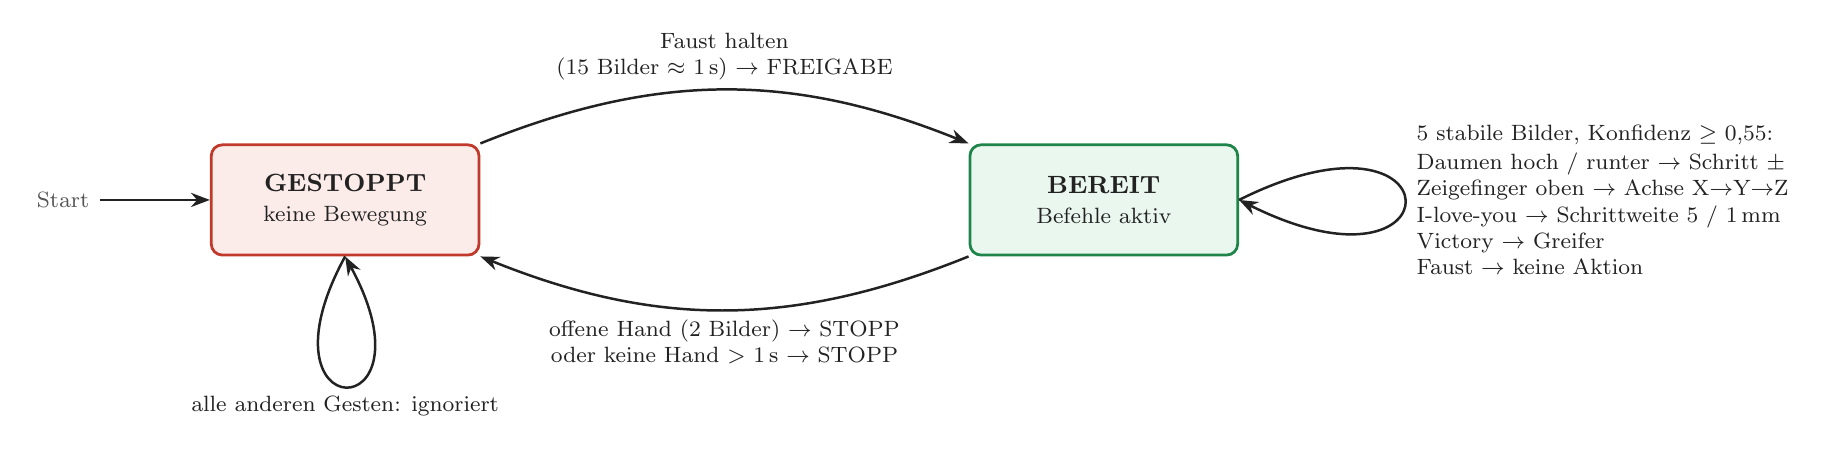
\begin{tikzpicture}[
  font=\small, >={Stealth[length=2.4mm]},
  zst/.style={draw, rounded corners=4pt, minimum width=34mm, minimum height=14mm, align=center, line width=1pt, text=tinte},
  pfeil/.style={->, line width=0.9pt, draw=tinte},
  lbl/.style={font=\footnotesize, text=tinte, align=center, fill=white, inner sep=2pt}
]
\node[zst, draw=rot, fill=rothell] (g) {\textbf{GESTOPPT}\\ \footnotesize keine Bewegung};
\node[zst, draw=gruen, fill=gruenhell, right=62mm of g] (b) {\textbf{BEREIT}\\ \footnotesize Befehle aktiv};
\draw[pfeil] ($(g.west)+(-14mm,0)$) node[left, font=\footnotesize, text=grau]{Start} -- (g.west);
\draw[pfeil] (g.north east) to[bend left=22] node[lbl, above=1pt]{Faust halten\\ (15 Bilder $\approx$ 1\,s) $\rightarrow$ FREIGABE} (b.north west);
\draw[pfeil] (b.south west) to[bend left=22] node[lbl, below=1pt]{offene Hand (2 Bilder) $\rightarrow$ STOPP\\ oder keine Hand $>$ 1\,s $\rightarrow$ STOPP} (g.south east);
\draw[pfeil] (b.east) .. controls +(28mm,14mm) and +(28mm,-14mm) .. node[lbl, right=2pt, align=left]{
  5 stabile Bilder, Konfidenz $\geq$ 0,55:\\[1pt]
  Daumen hoch / runter $\rightarrow$ Schritt $\pm$\\
  Zeigefinger oben $\rightarrow$ Achse X$\rightarrow$Y$\rightarrow$Z\\
  I-love-you $\rightarrow$ Schrittweite 5 / 1\,mm\\
  Victory $\rightarrow$ Greifer\\
  Faust $\rightarrow$ keine Aktion} (b.east);
\draw[pfeil] (g.south) .. controls +(-12mm,-22mm) and +(12mm,-22mm) .. node[lbl, below=1pt]{alle anderen Gesten: ignoriert} (g.south);
\end{tikzpicture}
\end{document}
